\chapter[Solución Propuesta]{Solución Propuesta} \label{sec:solucion_propuesta}

\section{Redefinición del Alcance y Objetivos del Proyecto}
Durante el transcurso del proyecto se identificaron una serie de restricciones de carácter económico, logístico y operativo que, en conjunto, tornaron inviable la ejecución del plan original en su totalidad. A continuación se describen los factores determinantes que motivaron la redefinición del alcance.

El plan original contempló el desarrollo de tres diseños de circuito impreso distintos: el amplificador de operación permanente en Clase AB, el amplificador de cresta en Clase C y los elementos pasivos de la topología Doherty. El costo unitario del transistor empleado, sumado a los costos de fabricación, envío y ensamblado de cada iteración de placa, representó una restricción económica significativa. Si bien las demoras asociadas al proceso de fabricación y envío desde el exterior fueron contempladas en la planificación original, la acumulación de estos tiempos a lo largo de tres iteraciones de fabricación habría comprometido seriamente el cronograma del proyecto. Adicionalmente, el ensamblado del primer circuito impreso fue realizado sin costo por parte de la empresa Outsource, beneficio que no podía garantizarse para las iteraciones subsiguientes, lo que introdujo una incertidumbre adicional tanto en los costos como en los plazos.

Desde el punto de vista del acceso a equipamiento de medición, el departamento de ingeniería electrónica de la facultad no contaba con el instrumental necesario para la caracterización de circuitos de radiofrecuencia a las frecuencias de trabajo consideradas en este proyecto. Para subsanar esta limitación se recurrió a la Comisión Nacional de Energía Atómica (CNEA) y a la Universidad Nacional de San Martín (UNSAM), instituciones donde se llevaron a cabo las mediciones. Sin embargo, el acceso a los equipos y a la ayuda por parte personal en dichas instituciones requirió coordinación anticipada y estuvo sujeto a la disponibilidad tanto de los integrantes del grupo como de las propias instituciones, lo que limitó no solo la frecuencia con que pudieron realizarse sesiones de medición, sino también el tiempo disponible dentro de cada sesión, dado que los equipos y los espacios de trabajo debieron compartirse con otras actividades propias de cada institución. Extender este esquema a la caracterización de tres diseños distintos habría requerido una cantidad y duración de sesiones de medición difícilmente compatible con los plazos disponibles.

En relación con los ensayos de irradiación contemplados en el anteproyecto, se presentaron dificultades para identificar una instalación experimental disponible cuyo tamaño de muestra admisible fuera compatible con las dimensiones del primer circuito impreso fabricado, el cual resultó de dimensiones superiores a las previstas inicialmente. Esta incompatibilidad física, sumada a la complejidad logística asociada a la coordinación de turnos de irradiación, llevó a desestimar la realización de este ensayo dentro del alcance del presente trabajo.

Frente a este conjunto de restricciones, y considerando que los resultados obtenidos en la caracterización del amplificador Clase AB, según se detalla en la Sección~\ref{sec:4_resmedver}, satisficieron en gran medida los objetivos de prestaciones establecidos en el anteproyecto, se tomó la decisión de redefinir el alcance del proyecto. El desarrollo quedó acotado al amplificador de potencia en Clase AB y al acoplador híbrido en cuadratura. El amplificador Clase AB constituyó por sí mismo un amplificador de potencia funcional que cumplió con gran parte de los requisitos de la misión, mientras que el acoplador híbrido representó una primera instancia de desarrollo que sentó las bases para una eventual continuación del trabajo hacia la implementación completa de la topología Doherty en el futuro. El ensayo de irradiación fue excluido del alcance actual, redirigiendo los esfuerzos hacia una caracterización experimental más exhaustiva de los parámetros del amplificador fabricado.

\section{Objetivo}
A partir del análisis comparativo de tecnologías semiconductoras desarrollado en la Sección~\ref{sec:gan_hemt} y de los criterios de diseño discutidos en la Sección~\ref{sec:teoria_pa}, se propuso el desarrollo de un amplificador de potencia monoetapa, basado en el transistor GaN HEMT CGH40006S, polarizado en Clase AB y destinado a operar en banda S sobre la frecuencia de portadora establecida de 2,2\,GHz para el enlace satelital de la misión CubeSat.

La elección de una topología de etapa única, en contraposición a una cadena de amplificación multietapa, se fundamentó en que la ganancia de pequeña señal característica del dispositivo seleccionado resulta suficiente para alcanzar la potencia de salida objetivo de la misión a partir de un nivel de excitación de entrada moderado, evitando así la complejidad adicional, el consumo de área de placa y los riesgos de estabilidad asociados al acoplamiento entre etapas sucesivas. Esta decisión es consistente con el criterio de simplicidad de implementación discutido al introducir la Clase AB como punto de polarización, dado que una topología de etapa única reduce significativamente el número de redes de adaptación de impedancia y de puntos de polarización independientes que deben diseñarse, simularse y ajustarse experimentalmente.

Esta cadena de decisiones de diseño no resulta arbitraria, sino que responde directamente a las restricciones impuestas por la plataforma CubeSat. La elección del GaN como tecnología semiconductora, fundamentada en la Sección~\ref{sec:gan_hemt} a partir de su elevada densidad de potencia y su figura de mérito de Johnson superior a la del silicio y el GaAs, permite alcanzar la potencia de salida requerida con un dispositivo de área reducida, minimizando la masa del disipador térmico necesario para mantener la temperatura de juntura dentro de límites admisibles en un volumen acotado. La operación en Clase AB, justificada en la Sección~\ref{sec:teoria_pa} a partir del compromiso entre linealidad y eficiencia que impone el esquema de modulación M-PSK adoptado para el enlace, se complementa con la selección puntual del CGH40006S, dispositivo cuya tensión de alimentación nominal de drain ($28$~V) resulta compatible con los niveles de tensión típicamente disponibles en el bus de potencia de una plataforma nanosatelital, evitando la necesidad de una etapa de conversión de tensión adicional dedicada exclusivamente al subsistema de radiofrecuencia. El consumo de potencia continua resultante, de aproximadamente $2{,}8$~W considerando la polarización nominal de drain y el consumo adicional de la polarización de gate, debe contemplarse dentro del presupuesto energético total disponible para la plataforma, el cual se encuentra acotado por la capacidad de generación fotovoltaica y de almacenamiento del sistema de potencia del CubeSat.

La validación de esta propuesta de diseño no se limita a la verificación mediante simulación de circuitos, sino que contempla la fabricación y caracterización experimental de un prototipo físico del amplificador, cuyos resultados de medición se presentan en una sección dedicada. Adicionalmente, dado que la potencia de salida de 1~W constituye un requisito derivado del balance de enlace satelital y no un valor arbitrario, se realizaron mediciones de radioenlace sobre el prototipo fabricado con el objetivo de determinar experimentalmente la tasa de bits máxima sostenible para los distintos esquemas de modulación M-PSK considerados, cerrando de esta manera el ciclo de diseño entre la especificación de la misión y el desempeño real del hardware desarrollado.

El desarrollo completo del amplificador, desde la etapa de diseño asistido por simulación hasta la fabricación y caracterización experimental del prototipo, se describe en las subsecciones siguientes. La Tabla~\ref{tab:objetivos_diseno} resume las especificaciones objetivo establecidas para el diseño, derivadas de los requerimientos de la misión y del balance de enlace satelital desarrollado en la Sección~\ref{sec:radioenlace}.

\begin{table}[H]
    \centering
    \caption{Especificaciones objetivo del amplificador de potencia.}
    \label{tab:objetivos_diseno}
    \begin{tabular}{lcc}
        \hline\hline
        \textbf{Parámetro}                   & \textbf{Valor Objetivo} & \textbf{Unidad} \\
        \hline
        Frecuencia central ($f_0$)           & 2,2                     & GHz             \\
        BW ($S_{11} < -10$ dB)               & $\ge$ 30                & MHz             \\
        $P_{out}$                            & $\ge$ 1                 & W               \\
        Ganancia de pequeña señal ($S_{21}$) & XX                      & dB              \\
        PAE                                  & $\ge$ XX                & \%              \\
        OIP3                                 & $\ge$ XX                & dBm             \\
        Factor de estabilidad ($\mu$)        & $> 1$ (incond.)         & ---             \\
        \hline\hline
    \end{tabular}
\end{table}

% -----------------------------------------------------------------------------------------------%
\section{Topología Propuesta}
La Figura~\ref{fig:diagrama_bloques} presenta el diagrama en bloques de la topología propuesta para el amplificador. La señal de entrada de radiofrecuencia ingresa a través de un filtro pasaaltos (HPF), seguido de una red bias tee que inyecta la polarización de gate ($-2{,}6$~V, $7$~mA) sin interferir con la trayectoria de la señal de RF, y de una red de estabilidad resistivo-capacitiva conectada en paralelo, dispuesta para extender la estabilidad incondicional del transistor hacia frecuencias por debajo de la banda de operación. A continuación, el transistor CGH40006S amplifica la señal, entregándola a un bloque de salida que integra de manera conjunta la adaptación de impedancia, el filtrado y la inyección de la polarización de drain ($28$~V, $100$~mA) mediante un filtro pasaaltos y una bias tee análogos a los de la entrada, antes de entregar la señal amplificada a la carga de $50\,\Omega$.

\begin{figure}[H]
    \centering
    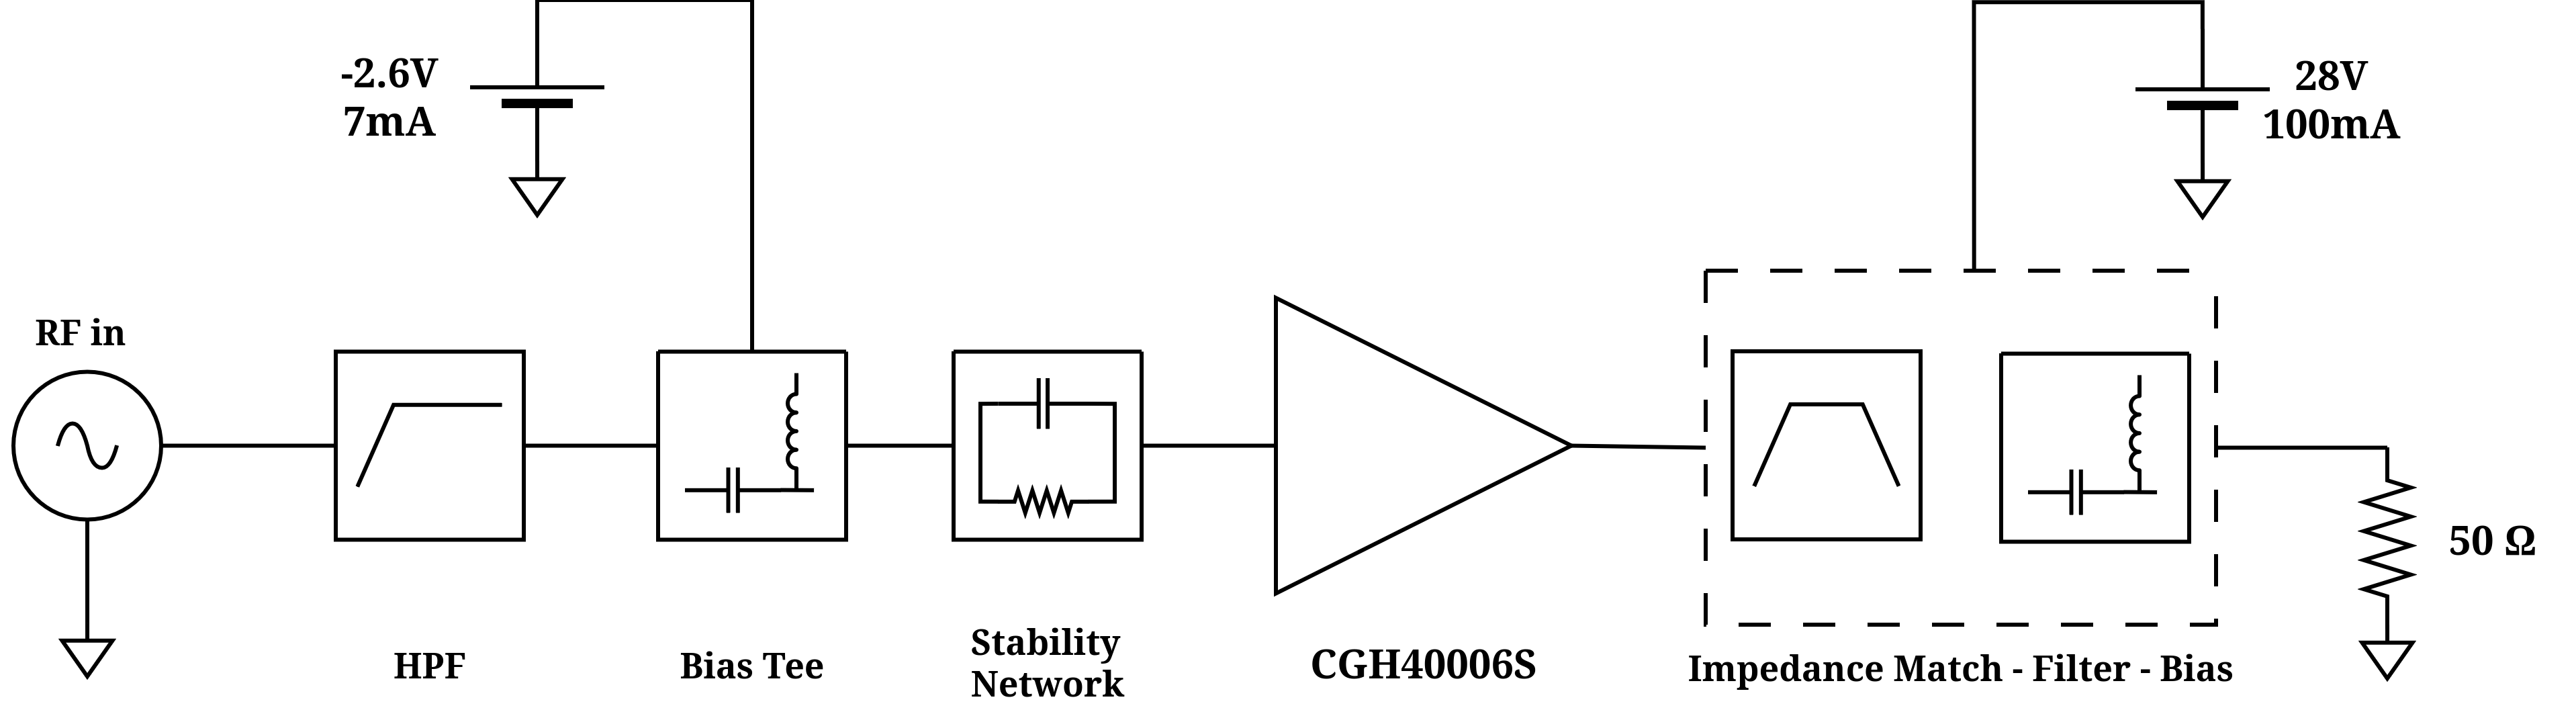
\includegraphics[width=\linewidth]{Figures/pa_block_diagram.png}
    \caption{Diagrama en bloques de la topología propuesta para el amplificador de potencia.}
    \label{fig:diagrama_bloques}
\end{figure}

% -----------------------------------------------------------------------------------------------%
\section{Transistor Seleccionado}
El transistor seleccionado para el diseño del amplificador de potencia fue el CGH40006S, un GaN HEMT discreto fabricado originalmente por Cree y comercializado actualmente por MACOM, encapsulado en formato de montaje superficial. La selección de este dispositivo se fundamentó en los siguientes criterios:

\begin{enumerate}
    \item \textbf{Especificaciones eléctricas adecuadas a la aplicación:} el dispositivo entrega una potencia de salida en el punto de compresión de 1~dB de aproximadamente 37{,}5~dBm a 2~GHz, con una ganancia de pequeña señal del orden de 20~dB y una eficiencia de potencia añadida cercana al 60\,\%, valores que exceden ampliamente el requisito de 1~W (30~dBm) de salida establecido para la misión, lo que otorga margen de diseño respecto del punto de compresión \cite{Macom}.

    \item \textbf{Disponibilidad de modelo no lineal del fabricante:} MACOM provee un modelo no lineal del CGH40006S compatible con entornos de simulación de circuitos de microondas, lo que permitió realizar simulaciones de gran señal del amplificador (compresión de potencia, distorsión de intermodulación, estabilidad) previas a la fabricación del prototipo físico, reduciendo el riesgo de iteraciones costosas en hardware.

    \item \textbf{Costo moderado dentro del segmento de GaN HEMT discretos:} al momento de redacción de este trabajo, el costo unitario del dispositivo se ubica en torno a los 75~USD, valor que se considera moderado para el segmento de transistores GaN HEMT discretos orientados a aplicaciones profesionales y aeroespaciales, en contraste con soluciones de mayor integración como los circuitos monolíticos de microondas (MMIC), cuyo costo y plazo de adquisición suelen ser sustancialmente mayores.

    \item \textbf{Aplicabilidad directa al proyecto:} la combinación de tensión de operación nominal de 28~V, compatible con los niveles de alimentación disponibles en la plataforma, y ganancia suficiente para alcanzar la potencia de salida objetivo con una única etapa de amplificación, simplificó la topología del circuito respecto de alternativas que hubiesen requerido múltiples etapas en cascada.
\end{enumerate}

% -----------------------------------------------------------------------------------------------%
\section{Metodología de Diseño y Simulación}
El diseño y la simulación del circuito se realizaron mediante el entorno Advanced Design System (ADS) de Keysight, empleando una biblioteca de modelos reales de componentes de montaje superficial (SMD) provista por los fabricantes correspondientes, en lugar de modelos ideales de elementos discretos. Sobre el esquemático de simulación se ejecutaron rutinas de optimización numérica para ajustar el ancho y el largo de las líneas de transmisión que conforman las redes de adaptación de entrada y de salida, hasta alcanzar las condiciones de adaptación de impedancia y de desempeño de gran señal requeridas en la frecuencia de operación.

A partir del esquemático optimizado se llevaron a cabo las siguientes simulaciones, cada una orientada a verificar un aspecto particular del comportamiento del amplificador:

\begin{itemize}
    \item \textbf{Parámetros $S$:} para caracterizar el comportamiento de pequeña señal del circuito completo, incluyendo las redes de adaptación, y verificar las condiciones de ganancia y de adaptación de impedancia en la banda de interés.
    \item \textbf{Estabilidad en entrada y en salida:} para verificar, mediante el factor $\mu$, definido en la Sección~\ref{sec:teoria_pa}, que el circuito completo se mantiene incondicionalmente estable tanto en la banda de operación como en frecuencias adyacentes, dado que las redes de adaptación y de polarización pueden introducir regiones de inestabilidad no presentes en el transistor.
    \item \textbf{\textit{Load-pull}:} para determinar la impedancia de carga óptima en el plano de Smith que maximiza simultáneamente la potencia de salida y la eficiencia del dispositivo, según se detalla más adelante en esta subsección. Adicionalmente, el software de simulación determina un valor adecuado para la impedancia de entrada que se complemente con el de carga.
    \item \textbf{Balance armónico (\textit{harmonic balance}) y contenido armónico:} para evaluar el comportamiento del circuito en régimen de gran señal en estado estacionario, obteniendo las curvas de compresión de potencia, ganancia, PAE y eficiencia de drain en función de la potencia de entrada, así como el nivel relativo de las componentes armónicas generadas por la no linealidad del transistor.
    \item \textbf{Transitorio en el dominio temporal:} para observar directamente las formas de onda de tensión y corriente en los terminales del transistor y en la carga adaptada a lo largo del ciclo de la señal, contrastando dichas formas de onda con el modelo de ángulo de conducción desarrollado en la Sección~\ref{sec:teoria_pa}.
\end{itemize}

Adicionalmente, se empleó el entorno de simulación electromagnética de campos High Frequency Structure Simulator (HFSS), también de Keysight, para verificar mediante simulación de onda completa el comportamiento de las estructuras de microstrip críticas del diseño, en particular en aquellas geometrías donde los efectos electromagnéticos parásitos no resultan adecuadamente capturados por los modelos analíticos de línea de transmisión empleados en el esquemático de ADS.

\textbf{Simulación de \textit{load-pull}.} El \textit{load-pull} es una técnica de caracterización de gran señal mediante la cual se barre sistemáticamente la impedancia de carga presentada al puerto de salida del transistor, mientras se mantiene fijo el nivel de excitación de entrada, registrando en cada punto del barrido el desempeño resultante del dispositivo. A diferencia de la adaptación conjugada empleada en pequeña señal, en la cual la impedancia óptima de carga se determina únicamente a partir de los parámetros $S_{22}$ del dispositivo, en gran señal la impedancia que maximiza la potencia de salida y la impedancia que maximiza la eficiencia no necesariamente coinciden entre sí ni con la impedancia conjugada de pequeña señal, debido a las no linealidades del transistor en la región de operación de interés.

El barrido de impedancias se realizó dentro de ADS utilizando el modelo no lineal del CGH40006S provisto por el fabricante, obteniendo como resultado un conjunto de contornos de potencia de salida constante ($P_{out}$) y de eficiencia de potencia añadida constante (PAE) trazados sobre el diagrama de Smith. Law intersecciones de estos contornos permitieron seleccionar una impedancia de carga de diseño como un compromiso entre ambos criterios, priorizando la región del plano de Smith donde ambas magnitudes se mantienen simultáneamente próximas a sus valores máximos, en lugar de optimizar exclusivamente alguna de las dos de forma aislada.

% -----------------------------------------------------------------------------------------------%
\section{Metodología de Diseño de PCB}
El diseño del circuito impreso (PCB) se realizó en el entorno Altium Designer, a partir de los modelos de las líneas de transmisión previamente dimensionadas y optimizadas en ADS, los cuales se exportaron y trasladaron al layout de la placa. Sobre dicho layout se incorporaron las vías de masa requeridas para garantizar la continuidad del plano de referencia y se configuró la estructura de capas (\textit{stackup}) de la placa de acuerdo con el proceso de fabricación JLC04161H-7628 del fabricante JLCPCB, una estructura de cuatro capas en sustrato FR4. La elección de este proceso específico se fundamentó en que ofrece impedancia controlada de $50\,\Omega$ como servicio estándar del fabricante, y en que había sido previamente empleado en proyectos previos con buenos resultados, lo cual permitió reutilizar parámetros de diseño y de fabricación ya validados experimentalmente con anterioridad. La Tabla~\ref{tab:pcb_stackup} detalla la estructura de capas resultante.

\begin{table}[b]
    \caption{PCB Stackup}
    \label{tab:pcb_stackup}
    \centering
    \renewcommand{\arraystretch}{1.1}
    \begin{tabular}{|l|c|c|}
        \hline
        \textbf{Capa} & \textbf{Permitividad Relativa (Dk)} & \textbf{Espesor} \\
        \hline
        Top      & \cellcolor{coppercolor}Copper  & 0.035mm   \\ \hline
        Prepreg  & \cellcolor{dielectriccolor}4.4 & 0.21040mm \\ \hline
        Inner L2 & \cellcolor{coppercolor}Copper  & 0.0152mm  \\ \hline
        Core     & \cellcolor{dielectriccolor}4.6 & 1.065mm   \\ \hline
        Inner L3 & \cellcolor{coppercolor}Copper  & 0.0152mm  \\ \hline
        Prepreg  & \cellcolor{dielectriccolor}4.4 & 0.21040mm \\ \hline
        Bottom   & \cellcolor{coppercolor}Copper  & 0.035mm   \\
        \hline
    \end{tabular}
\end{table}

El diseño del layout de RF incorporó un conjunto de criterios y prácticas recomendadas para minimizar las pérdidas y las desadaptaciones parásitas inherentes a la implementación física del circuito:

\begin{itemize}
    \item Los caminos de señal de radiofrecuencia se trazaron de la forma más rectilínea posible, evitando curvas y quiebres innecesarios que pudieran introducir desadaptaciones de impedancia.
    \item La separación entre pistas de señal, y entre pistas y el plano de masa adyacente, se estableció en al menos cinco veces el espesor del dieléctrico correspondiente, con el objetivo de evitar acoplamiento electromagnético indeseado entre conductores próximos.
    \item Las distancias entre vías de masa se mantuvieron por debajo de $\lambda/10$ en la frecuencia de operación, con el objetivo de evitar la aparición de acoplamiento parásito entre vías adyacentes, y se emplearon múltiples vías en paralelo en los puntos críticos de conexión a masa con el fin de reducir la inductancia parásita asociada.
    \item Se prestó especial atención al acople de masa en dos zonas consideradas críticas para el correcto funcionamiento del circuito: el conector SMA, cuyo estándar de conexión exige un acople de masa adecuado para garantizar la continuidad de la referencia entre el conector y la placa, y la masa del transistor, dado que un acople deficiente en este punto incrementa la inductancia parásita de source y degrada tanto la ganancia como la estabilidad del dispositivo.
    \item Las líneas de transmisión que no requerían un valor de impedancia específico para el funcionamiento del circuito se diseñaron con impedancia característica de $50\,\Omega$, manteniendo consistencia con la impedancia de referencia del sistema y de los instrumentos de medición.
    \item El orden de montaje de los capacitores de filtrado de las fuentes de polarización se estableció de acuerdo con su valor de capacitancia, ubicando el capacitor de mayor valor más próximo a la fuente de alimentación, dado que su frecuencia de autorresonancia resulta más baja que la de los capacitores de menor valor, los cuales se ubicaron progresivamente más cerca del transistor para filtrar las componentes de mayor frecuencia.
\end{itemize}

Dado que el diseño correspondía a una primera versión de desarrollo, y considerando la disponibilidad limitada de únicamente dos unidades del transistor para la totalidad del proyecto, el layout se concibió con el objetivo de habilitar la mayor cantidad posible de mediciones y ajustes experimentales sobre la misma placa fabricada. Con este fin, se incorporaron \textit{pads} adicionales sin conexión eléctrica que permiten, en caso de ser necesario, extender la longitud de los \textit{stubs} de las redes de adaptación (Figura~\ref{fig:stubs_ajustables}) o modificar el ancho de las líneas de transmisión (Figura~\ref{fig:txlines_ajustables}) mediante la incorporación manual de puentes de soldadura, sin requerir una nueva iteración completa de fabricación de la placa.

\begin{figure}[H]
    \centering
    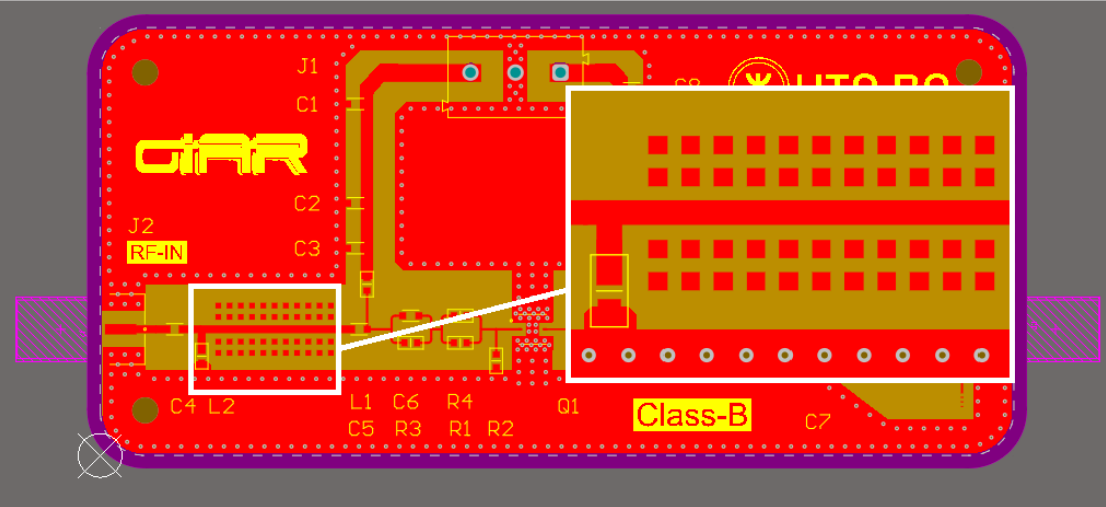
\includegraphics[width=\linewidth]{Figures/pcb_stubs_extra.png}
    \caption{Pads adicionales incorporados para permitir la extensión de la longitud de los stubs de adaptación, en caso de requerirse ajuste experimental.}
    \label{fig:stubs_ajustables}
\end{figure}

\begin{figure}[H]
    \centering
    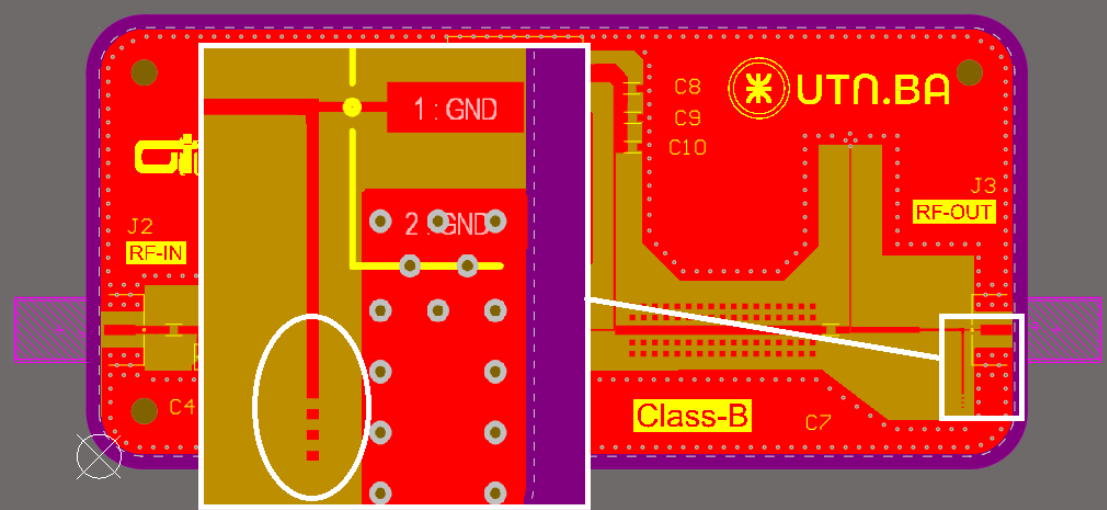
\includegraphics[width=\linewidth]{Figures/pcb_ltx_extra.png}
    \caption{Pads adicionales incorporados para permitir la modificación del ancho de las líneas de transmisión, en caso de requerirse ajuste experimental.}
    \label{fig:txlines_ajustables}
\end{figure}

% TODO: consultar si poner los nombre o hablar de forma genérica
Una vez finalizada la etapa de diseño del layout, se realizó una consulta con el docente Carlos Navarro con el objetivo de obtener una revisión externa del diseño. Si bien dicha revisión no constituyó un análisis exhaustivo del circuito, permitió confirmar que los criterios de diseño adoptados, así como los valores de tolerancia de tensión considerados, se encontraban dentro de las prácticas recomendadas para este tipo de circuitos de radiofrecuencia, y resultó de utilidad para resolver dudas puntuales surgidas durante el proceso de diseño.

% TODO: buscar compañia y si la ponemos o no, creo que era outsource
Finalmente, se solicitó la fabricación de la placa junto con un stencil, con el objetivo de enviar el ensamblado de los componentes de montaje superficial a una empresa de servicios de soldadura.

% -----------------------------------------------------------------------------------------------%
\section{Metodología de Medición}
Para validar experimentalmente el diseño propuesto, se llevó a cabo un conjunto de mediciones que abarcan el comportamiento de pequeña señal, el desempeño de potencia en gran señal y la caracterización no lineal del amplificador. Debido a la falta de equipamiento disponible en la universidad para realizar mediciones de armónicos o frecuencias superiores a los 3\,GHz, no fue posible llevar a cabo la totalidad de las mediciones dentro de las instalaciones de la institución. Por este motivo, se recurrió a la colaboración de ayudantes de cátedra que se desempeñan profesionalmente en la Comisión Nacional de Energía Atómica (CNEA), quienes facilitaron el acceso a los equipos necesarios y asistieron durante las mediciones de parámetros de dispersión, potencia de salida y OIP3, principalmente mediante el uso del PNA y el sensor de potencia disponibles en dicha institución. Esta colaboración estuvo a cargo del Dr.~Manuel García Redondo y el Dr.~Matías Hampel. Las mediciones de distorsión armónica, por su parte, se realizaron en las instalaciones de la Universidad Nacional de San Martín (UNSAM), con la asistencia del Ing.~Sanca. Cada medición requirió un setup dedicado, descrito en las siguientes subsecciones.

% -----------------------------------------------------------------------------------------------%
\subsubsection{Medición de Parámetros de Dispersión}
Los parámetros de dispersión se midieron con el objetivo de validar el diseño de las redes de adaptación y caracterizar el comportamiento de pequeña señal del amplificador. Se empleó un analizador de redes vectorial (VNA) Keysight N5242B PNA-X, calibrado mediante el método TOSM con un kit de calibración Keysight 85052B. En el puerto de salida se insertaron en cascada un atenuador de 20\,dB y otro de 10\,dB con el fin de proteger el receptor del VNA frente a los niveles de potencia elevados presentes a la salida del amplificador. En consecuencia, únicamente se reportan los parámetros $S_{21}$ y $S_{11}$, dado que la presencia del atenuador en el puerto de salida impide una medición confiable de los parámetros que involucran la reflexión hacia dicho puerto. El valor medido de $S_{21}$ fue corregido sumando el valor nominal del atenuador.

% -----------------------------------------------------------------------------------------------%
\subsubsection{Medición de Potencia de Salida}
Se realizó una medición de potencia de salida con el fin de caracterizar el comportamiento de gran señal del amplificador. Dado que el dispositivo bajo prueba requiere niveles de excitación superiores a la potencia de salida que el VNA es capaz de entregar, se insertó un amplificador driver Mini-Circuits ZX60-83LN12+ entre la fuente de señal del Keysight N5242B y el amplificador de potencia bajo prueba. La potencia de salida se midió con un sensor de potencia Keysight U8485A, precedido por un atenuador de 20\,dB y un atenuador de 10\,dB. La potencia de entrada se barrió en pasos de 2,5\,dBm a la frecuencia nominal de operación de 2,2\,GHz. Los valores obtenidos mediante esta medición se emplearon para determinar la ganancia y el punto de compresión de 1\,dB del amplificador.

Dado que el amplificador driver ingresa en compresión dentro del rango de medición, el punto de compresión de 1\,dB del dispositivo bajo prueba no puede obtenerse de forma directa a partir de la curva de potencia de salida medida. Por este motivo, se aplicó la expresión de compresión en cascada de la ecuación~\eqref{eq:p1db_cascada}, que refiere la compresión de cada etapa a la entrada del sistema y combina sus contribuciones ponderadas inversamente por la ganancia de las etapas precedentes

\begin{equation}
\frac{1}{P_{\text{1dB},sys}} = \frac{1}{G_2 \cdots G_N \, P_{\text{1dB},1}} + \frac{1}{G_3 \cdots G_N \, P_{\text{1dB},2}} + \cdots + \frac{1}{P_{\text{1dB},N}}
\label{eq:p1db_cascada}
\end{equation}

% -----------------------------------------------------------------------------------------------%
\subsubsection{Medición de Distorsión Armónica}
Debido a la no linealidad intrínseca de todo dispositivo activo, sumada a la clase de operación en la que se polariza el amplificador, las etapas de potencia generan distorsión armónica que degrada la pureza espectral de la señal y puede provocar interferencia fuera de banda. Para caracterizar este comportamiento, se midieron el segundo y el tercer armónico utilizando un generador de señal Siglent SSG3032X-IQE como fuente de excitación de onda continua a 2,2\,GHz y un analizador de espectro Keysight N9322C a la salida. Se colocó un atenuador de 20\,dB en la entrada del analizador con fines de protección. La potencia de entrada se barrió desde 0\,dBm hasta 20\,dBm en pasos de 5\,dBm.

% -----------------------------------------------------------------------------------------------%
\subsubsection{Medición de OIP3}
El punto de intercepción de tercer orden a la salida (OIP3) se obtuvo mediante la aplicación de software ``IMD Sweep'' (S93087B IMD) del VNA Keysight N5242B PNA-X. De forma análoga a la medición de potencia de salida, se incorporó el amplificador driver Mini-Circuits ZX60-83LN12+ entre la fuente de señal del VNA y el dispositivo bajo prueba, con el fin de capturar adecuadamente los efectos de gran señal. Asimismo, se agregaron dos atenuadores de 20\,dB y 10\,dB a la salida del dispositivo bajo prueba para proteger los puertos del VNA. La separación de frecuencia entre los dos tonos se fijó en 10\,MHz, con una potencia de cada tono de $P_{in} = -5\,\text{dBm}$.